\documentclass[12pt, a4paper]{article}
\usepackage{hyperref}
\usepackage{pgfplots}
\usepackage{graphicx}
\graphicspath{ {./Files/} }

\title{Group19 Project 5: A P2P File Sharing Program}
\author{Nicholas van Huyssteen, Lehann Smith\\
    \small{20869118@sun.ac.za, 19027176@sun.ac.za}
}
\date{23 October 2019}

\begin{document}

\maketitle

\section{Introduction}
The purpose of this project was to implement a peer-to-peer file sharing program with a central mediating server. This project involved solving problems in the realms of encryption, key-passing, threading, file transfer and server-client communication.
The final program is comprised of a server-client model during initial communication. The server acts as a mediator between different clients. The server "introduces" clients. The second significant stage of communication involves clients passing keys to verify identity, the encryption and decryption of information and file transfer via TCP-socket communication.

\section{Program Description}
\paragraph{A General Overview:}
The program makes use of both a server-client model and peer to peer communication. Clients connect to the server to send messages, search for files or make their files available. The server distributes and processes search requests. Download requests are mediated by the server (the relevant clients are introduced and addresses are passed along). If a request is accepted, the server ceases to be an interloper between the clients. Instead, the clients open a direct line of communication to exchange public keys and verify keys. If all checks are passed, the specified file is sent to the requesting client.

\paragraph{Starting and Set-up of the Server}
Simply run StartServer. This sets up a server with the address of the computer it runs on.

\paragraph{Starting and Set-up of the Client}
Run StartClient as './StartClient x', where x is the address of the server as a String. This launches ClientInitGUI, and upon successfully connecting to the server with a valid username, it launches an instance of the client.

\paragraph{Connecting Clients}
After running StartClient, which calls ClientInitGUI, a connection is made with the server, however only once a valid username is submitted, does the server add this instance of the client to the list of currently active clients, which is effectively the pathway through which the server recognizes the validity of the clients.

\paragraph{Download Requests and Key Passing}
When a user selects a file (and thereby the client who owns that file) a download request is sent and verified from the receiving user (A) to the sending user (B). The request is sent to the server from A. The server passes on the request to B. In the first phase public keys and addresses are exchanged between the users. User A will send an instance of TCPObject tagged as a pre-download request to the server. The server will identify B based on the nickname supplied in the object and pass it on to B. B will receive A's public key and sends its own public key back through the same process. A random key is generated by the user A using the Keys class. This random key is sent inside a TCPObject (containing the nickname of the user A, the nickname of user B, the filename and the encrypted key) to the server. The server then adds the address of user A to this object, and sends the whole object to user B. Using the supplied address, tentative communications are opened directly between user A and B. The file sending user (B) decrypts the random key and sends it back to the receiving user (A) to be checked. If the key is correct file sending may commence.

\paragraph{Downloading}
The clients set up a TCP connection using the information acquired from the TCPObject in the download request step. The clients exchange public keys and pertinent file information (such as the filename, the number of chunks it will be broken up into, the size of the chunks and the size of the final chunk). The receiver receives every chunk, decrypts the chunk and writes it to an output file.
After every chunk that is received, the client updates its current progress (the number of chunks that it has received divided by the total number of chunks it is expecting to receive as transmitted in the file information transfer). The client writes a boolean after every chunk to the sending user that indicates if it wants the sending user to keep writing to the stream. This boolean is set to false if the user has pressed the pause button.

\paragraph{Uploading}
The clients set up a TCP connection. The clients exchange public keys and pertinent file information(such as the filename, the number of chunks it will be broken up into, the size of the chunks and the size of the final chunk). The sender breaks the file into byte array chunks, encrypts the chunks and writes them to the receiver. After every chunk is sent, the current progress (the number of chunks sent divided by the total number of chunks) is updated and a boolean is read over TCP from the receiving client. This boolean indicates whether the receiving client has paused the download. If the boolean is false, the client will continuously wait to receive the signal that it may continue writing to the stream.

\paragraph{Searching}
Searching is done by computing the Levenshtein number between a supplied search term and the names of the files owned by the client. A specified tolerance number (calculated based on the length of the word) is used to filter the results. All results within the tolerance will be returned to the searching client. The client sets up an array with either a single entry: "empty", or populates the array the filenames of every file within the acceptable parameters. This array is sent back to the server via an instance of the TCPObject to be routed back to the originals searching client.

\paragraph{Encryption}
Diffie Hellman symmetric key encryption is used in the implementation of this project. A symmetric block cipher is used by our method of encryption, namely the AES standard. Encryption and decryption takes place on the client-side. Communication between the clients and the server happens in the TCPObject classes that are passed. This object has a type field that the server uses to distinguish what kind of action needs to be taken to process the message. A few other fields depending on the object is also visible to the server to assist in routing the objects, such as the name of the user the message is from. When private communication happens between clients after the server has "introduced" them, an instance of this class is also used. The clients pass read/write instances of these objects (with encrypted contents and visible fields) during the file transfer. Encryption happens in two prominent places. The contents of the byte chunks (the file contents itself) are encrypted before sending the chunk. In addition, the random key generated during the download request is encrypted. For the encryption of the file, public keys are exchanged directly between clients before the file is sent. In the case of the randomly generated key, public keys are generated and sent via a special instance of the TCPObject class via the server.

\section{File(s) Description}
\paragraph{Server}
The server is a program that is always active in the background and coordinates (and in some cases relays) the network activities of the clients. It is responsible for handling new client connections, client disconnections, maintaining a list of active clients and their respective information (usernames, sockets, etc.), and coordinating the establishment of connections between clients for file sharing.

\paragraph{Client}
The Client class hosts a slew of methods that interacts with the server, as well as a run method that awaits responses from the server, as necessary for further computation. An instantiation of a client saves the client's relative information such as its username and socket object. The usual client-server interaction starts with calling a client method that sends an object to the server, it then awaits and eventually receives a response object containing data necessary data for further computation.

\paragraph{ClientInitGUI}
This class functions as the starting point for the client-side program. Upon running it, it simultaneously spawns a window that requests a username from the user and connects to the server of the specified address given as an input parameter. The client can then submit a username, and if that username is valid (Not an empty string and isn't already in use by a client connected to the server) it launches ClientGUI.

\paragraph{ClientGUI}
This class functions as the front-end interface for the user to be able to take advantage of the functionality and methods that the client class offers. It also shows a list of the currently active clients. It features frame scalability without visual artifacts upon window resizing.

\includegraphics{universe}

\paragraph{BasicSender}
BasicSender is the class that sends the requested file to the receiving user during the peer to peer communication after the server has introduced them. This class contains several significant methods, namely sendChunkData(), sendFile(), and sendChunk().

sendChunkData() receives the public key from the sending user. This key will be used in encrypting the chunks before sending them. This method also writes the name of the file, the sizes of the individual and last chunks, and the number of chunks that the receiver can expect to the stream.

sendFile() reads the file into byte arrays that it sends to the receiver. It reports on the current progress of the upload and continually checks if the receiving user has paused its download. If it has, it holds off on writing more chunks until it receives the unpause boolean

sendChunk() reads the next chunk from the file, encrypts the chunk and writes it to the receiver.

\paragraph{BasicReceiver}
BasicReceiver is the class that receives the requested file during the peer to peer communication. This class contains several significant methods, namely recvChunkData(), recvFile(), and recvChunk(). Further, it also contains the methods necessary to pause and resume the download and report on the progress of the current downloading file.

recvChunkData() receives the public key from the sending user to be used in decrypting the partial file data that it has received. It then sends its public key back to the sending user. This method also receives the name of the file, the sizes of the individual and last chunks, and the number of chunks that it can expect.

recvFile() sets up the streams, file paths, and extensions to be written to. It then waits to receive the pre-determined number of chunks and reports on the progress of the download while it does so.

recvChunk() is the method that receives every individual encrypted chunk, decrypts it and writes the chunk to the file. After every received chunk it signals the sender whether or not it may continue to send.

\paragraph{TCPObject}\label{sec:TCPObject}
The TCPObject class was used in practically all communication. It features several subclasses with specific purposes. For example, a message class, a searchResults class, and a downloadRequest class. These classes are identified by the type field and processed by the server/client accordingly. The different subclasses are further differentiated by specific fields, ie the downloadRequest class has a field for the filename and a field for the nickname of the user requesting the file. These objects are transferred over the TCP sockets between the server and the clients.

\paragraph{DHEncryption}
This class drives the encryption of byte arrays. It uses symmetric encryption in the form of the AES standard. It makes use of the javax.crypto suite to generate a public key for every user and compute shared secrets after receiving the public key of the sending user. It contains the encryptMessage() and decryptMessage() methods. encryptMessage() takes an unencrypted byte array as input and returns the new encrypted byte array. decryptMessage() takes an encrypted array and returns the decrypted array.

\paragraph{Keys}
This class is responsible for generating a random key (a byte array consisting of 12 characters ranging from the byte values of 0-9/A-Z ) to be used in the download request verification.

\paragraph{SearchFile}
This class drives the search function. The class takes an input string (the search term) and an array of strings (the files to be matched). The most important method in the class is testForMatch(int tolerance). It uses the Levenshtein class (see below) to compute the distances between the search term and every item in the array. It returns an array containing every result that had a Levenshtein distance less than or equal to the tolerance parameter. If no results are found an array with a single "empty" result is returned.

\paragraph{Levenshtein}
This class takes two strings as input and returns the Levenshtein distance (\href{https://en.wikipedia.org/wiki/Levenshtein_distance}{Levenshtein.wiki}) between them. This distance represents how close of a match the two strings are.

\section{Experiments}
A simple modification was made in the source code of the program to measure the elapsed time for the sending and receiving of files. This allows for the ability to measure the time it takes to send a file relative to other variables as shown in the experiments below.

\subsection{Experiment 1: Varying file sizes with a constant packet size and measuring down/upload times}
\paragraph{Hypothesis:}
The time taken to send a file given constant packet size will increase linearly with the file size.
\paragraph{Method:}
Permutation 1: Fix the packet size at 100KB. Attempt to send files of increasing size (1-, 5-, 10-, 50-, 100- MB) and measure the wall-clock time right before the first packet to right after the last packet. Sending is one-way, ie client A downloads and client B uploads. Observe a relationship between the file size and the time taken to download the file. 
Permutation 2: Fix the packet size at 100KB. Attempt to send files of increasing size (1-, 5-, 10-, 50-, 100- MB) and measure the wall-clock time right before the first packet to right after the last packet. Sending is concurrent, ie client A downloads from client B and simultaneously uploads to client B. Similarly, client B uploads to client A and downloads from client A simultaneously. Observe a relationship between the file size and the time taken to download the file.
\paragraph{Results:} 

\begin{center}
\caption{packet size: 100 KB, time (ms)}\\
\begin{tabular}{ |c|c| }
    \hline
    \multicolumn{2}{|c|}{Permutation 1: single way send/receive} \\
   \hline
   File Size: & Download \\
   \hline
   1MB &454 \\
   \hline
   5MB&2111 \\
   \hline
   10MB&4340 \\
   \hline
   50MB&21061 \\
   \hline
   100MB&41915 \\
   \hline
\end{tabular}
\end{center}

\begin{center}
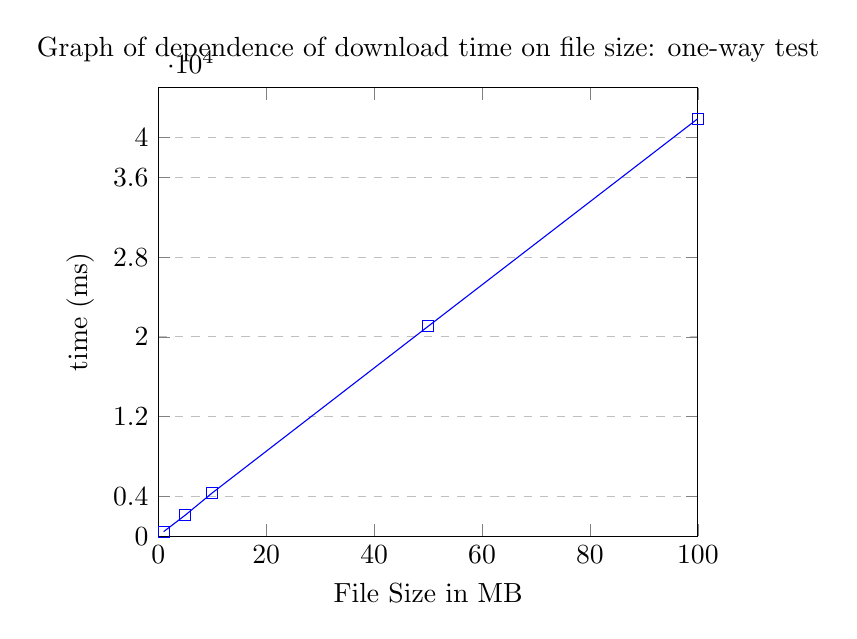
\begin{tikzpicture}
\begin{axis}[
    title={Graph of dependence of download time on file size: one-way test},
    ylabel={time (ms)},
    xlabel={File Size in MB},
    ymin=0, ymax=45000,
    xmin=0, xmax=100,
    ytick={0,4000,12000,20000,28000,36000, 40000},
    xtick={0,20,40,60,80,100},
    ymajorgrids=true,
    grid style=dashed]
\addplot[
    color=blue,
    mark=square,
    ]
    coordinates {
    (1, 454)(5, 2111)(10, 4340)(50, 21061)(100, 41915)
    };
\end{axis}
\end{tikzpicture}
\end{center}

\begin{center}
\caption{packet size: 100 KB, time (ms)}\\
\begin{tabular}{ |c|c| }
    \hline
    \multicolumn{2}{|c|}{Permutation 2: concurrent send/receive}\\
   \hline
   File Size: & Download \\
   \hline
   1MB &422\\
   \hline
   5MB&2149 \\
   \hline
   10MB&4236 \\
   \hline
   50MB&21023\\
   \hline
   100MB&42076 \\
   \hline
\end{tabular}
\end{center}

\begin{center}
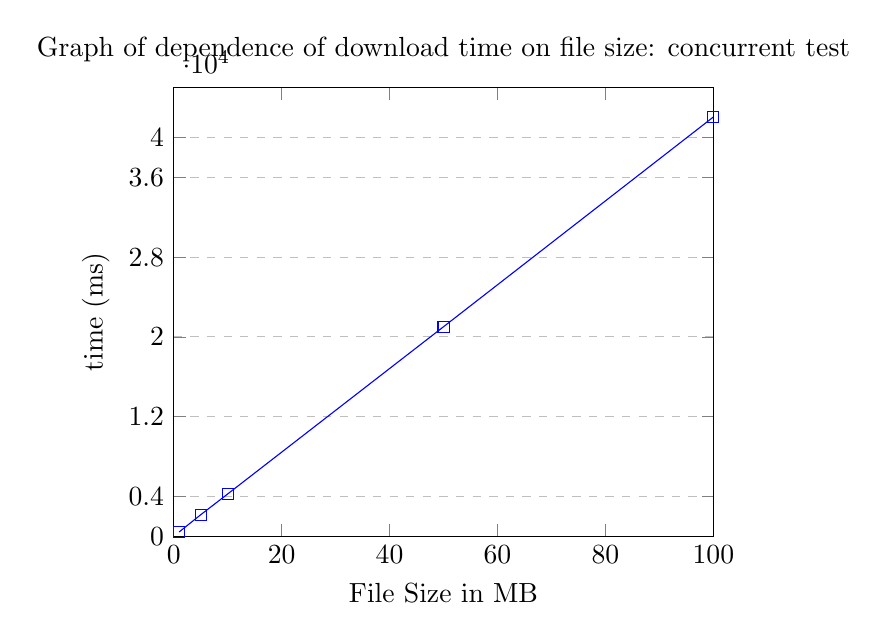
\begin{tikzpicture}
\begin{axis}[
    title={Graph of dependence of download time on file size: concurrent test},
    ylabel={time (ms)},
    xlabel={File Size in MB},
    ymin=0, ymax=45000,
    xmin=0, xmax=100,
    ytick={0,4000,12000,20000,28000,36000, 40000},
    xtick={0,20,40,60,80,100},
    ymajorgrids=true,
    grid style=dashed]
\addplot[
    color=blue,
    mark=square,
    ]
    coordinates {
    (1, 422)(5, 2149)(10, 4236)(50, 21023)(100, 42076)
    };
\end{axis}
\end{tikzpicture}
\end{center}

\paragraph{Conclusions:}
We observe that our hypothesis hold for the values tested. A clear linear relationship is observed between the file size and the measured download times. We can conclude from this observation that no meaningful computational overhead is added at large file sizes. This is consistent with our expectations given that the file is broken up into chunks instead of loaded into memory. The performance penalty added by encryption/decryption does not scale adversely with file size but remains constant. No relatively large download times are observed for very small files. We can further conclude that if there exists significant computational overhead that forms a larger part of the total execution time, it must take place before sending (the exchanging of the keys, set up of streams) or after receiving the chunks.

\subsection{Experiment 2: Varying packet sizes with a constant file size and measuring down/upload times}
\paragraph{Hypothesis:}
The time taken to send a file given constant file size will exhibit an inverse relationship with the packet size.
\paragraph{Method:}
 Fix the file size at 50MB. Attempt to send the files using increasing packet size (10-, 50-, 100-, 1024-, 5120- KB) and measure the wall-clock time right before the first packet to right after the last packet. Sending is one-way, ie client A downloads and client B uploads. Observe a relationship between the packet size and the time taken to download the file. 
\paragraph{Results:} 

\begin{center}
\caption{file size: 50 MB, time (ms)}\\
\begin{tabular}{ |c|c| }
   \hline
   File Size: & Download \\
   \hline
   1MB &422\\
   \hline
   5MB&2149 \\
   \hline
   10MB&4236 \\
   \hline
   50MB&21023\\
   \hline
   100MB&42076 \\
   \hline
\end{tabular}
\end{center}

\begin{center}
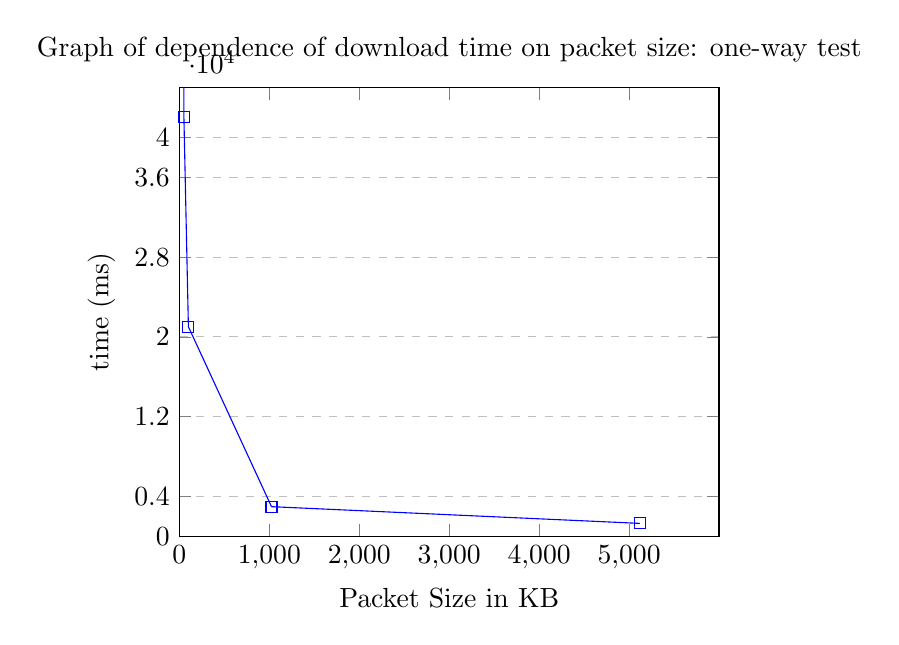
\begin{tikzpicture}
\begin{axis}[
    title={Graph of dependence of download time on packet size: one-way test},
    ylabel={time (ms)},
    xlabel={Packet Size in KB},
    ymin=0, ymax=45000,
    xmin=0, xmax=6000,
    ytick={0,4000,12000,20000,28000,36000, 40000},
    xtick={0,1000,2000,3000,4000,5000},
    ymajorgrids=true,
    grid style=dashed]
\addplot[
    color=blue,
    mark=square,
    ]
    coordinates {
    (10, 210978)(50, 42075)(100, 21023)(1024, 2963)(5120, 1285)
    };
\end{axis}
\end{tikzpicture}
\end{center}



\paragraph{Conclusions:}
We observe that an inverse exponential relationship can be observed between the packet size and the time taken to send the file. This suggests that the program becomes more efficient at larger packet sizes. We have to adjust our hypothesis to reflect this exponential scaling. This increase can be attributed to the computational overhead involved the steps of sending each file in effect becoming a relatively smaller proportion of the total send time. A smaller packet size means the file is being broken up into more individual chunks, which in turn leads to more calls to the encryption/decryption class. A larger packet size and therefore a smaller number of chunks means there are fewer calls to methods that add overhead. These methods include the continuous updating of the keepSending boolean, encryption/decryption of the bytes, the reports on the progress of the download/upload and the calls to the file-writer. We expect this trend to reverse at truly large packet sizes, as the performance degradation due to memory usage will eventually start to outweigh the reduced overhead.

\section{Issues Encountered}
We encountered an issue during the encrypting of the randomly generated key that is passed before the download is initiated. Because the users have not established private communication at this point, exchanging public keys is a fairly lengthy process of sending TCPObjects with the relevant information through the server until the encryption has been set up.

A further issue was encountered during the first iteration of folding encryption into the implementation. Originally the random key was generated as a string. This string was encrypted and sent via the sockets and attempted to be decrypted. However, the encoding differences between the original input string and the string received by the client enacted by reading and writing through the sockets meant that the received key was not recognized as equal in either length or contents to the original key. This was solved by moving encrypting/decrypting to a byte array-based implementation instead of strings. Similarly, encrypting the file chunks as byte arrays and sending the byte arrays circumvented the differences in the sent and received contents.

\section{Significant Data Structures}
We made use of ArrayLists to store the list of connected clients on the server-side.
Further use was made of a concurrent hashmap to store the ClientHandlers responsible for server-client communication.

The TCPObject class with its various subclasses occupied a pivotal role in our implementation. Almost all communication made use of an instance of this class. For further explanation for the class and its role see TCPObject: \ref{sec:TCPObject}.

\section{Design}
We decided to make use of Levenshtein numbers instead of Trigram, Jaro-Winckler or another string similarity algorithm due to ease of implementation, being able to better display the results of the algorithm in an intuitive format. Another consideration was that accounting for transposition of characters in the searched for terms overhead. The additional overhead in the search time outweighed the ease of search that would be gained in including transpositions.


\section{Compilation}
In the repository-directory, open a terminal and run the script ./StartServer.sh (external IP of the local machine) to compile and run a Server on the local address. Run ./StartClient.sh to run a client. Input the client nickname when prompted to connect to the server.

\section{Execution}
In the repository-directory, open a terminal and run the script ./StartServer.sh (external IP of the local machine) to compile and run a Server on the local address. Run ./StartClient.sh to run a client. Input the client nickname when prompted to connect to the server. the server.

\section{Libraries}
We made use of javax.crypto and java.security during encryption and random key generation. On the tutorialspoint website, we found an example of the encryption style we used (\href{https://www.tutorialspoint.com/java_cryptography/java_cryptography_encrypting_data.htm}{Tutorialspoint Crypto}). We adjusted it to work with byte arrays instead of strings as per the example. Further, the pseudo-code for the algorithm to compute the Levenshtein number was obtained from the Wikipedia page on Levenshtein distance: \href{https://en.wikipedia.org/wiki/Levenshtein_distance}{Levenshtein.wiki}.
We made extensive use of the java.util.concurrent library for out data structures and the JavaFX library in the construction of the GUI.

\end{document}
